\chapter{Evaluierung}\label{kap:eval}

\section{Evaluierungs Metriken}\label{sec:metricen}

\subsection*{Mean Average Precision (mAP)}

Als Metrik für die Genauigkeit eines Object Detection Models 
dient die \textit{Mean Average Precision (mAP)}, welche 
sowohl Klassifizierung als auch Lokalisierung mit einbezieht 
und sich aus folgenden Werten berechenn lässt.


\begin{itemize}
  \item \textit{True Positive (TP)}: 
  \item \textit{True Negative (TN)}: 
  \item \textit{False Positive (FP)}: 
  \item \textit{False Negative (FN)}: 
\end{itemize}

Zur bestimmung von TPs wird die \textit{Intersection over unioun}
verwendet, welche Überlappungsgrad der gelabelten (Ground Truth) und der
geschätzete Boundig Box zu dem Gesammtbereich beider Boxen darstellt 

Beträgt dieser mehr als ein Bestimmter Threshhold, häufig 50\%
gilt die Schätzung als \textit{True Positive}, andernfalls als 
\textit{False Positive}. 


% für confusion matrix
\newcommand\MyBox[2]{
  \fbox{\lower0.75cm
    \vbox to 1.7cm{\vfil
      \hbox to 1.7cm{\hfil\parbox{1.4cm}{#1\\#2}\hfil}
      \vfil}%
  }%
}
\noindent
\renewcommand\arraystretch{1.5}
\setlength\tabcolsep{0pt}

\begin{minipage}{\textwidth}
    \begin{minipage}[b]{0.49\textwidth}
      \centering
      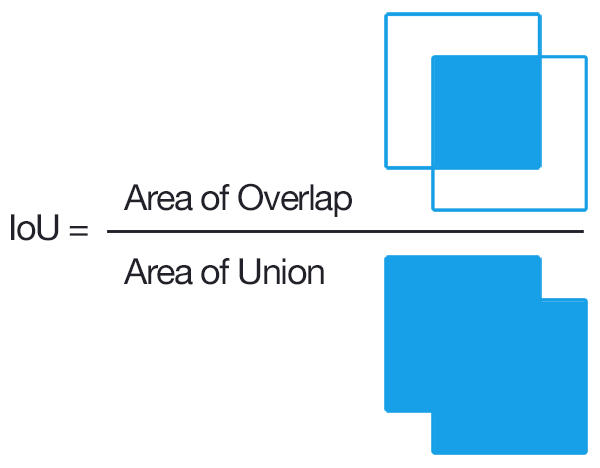
\includegraphics[width=0.8\textwidth]{Bilder/IoU.png}
      \captionof{figure}{Intersection over Union}
    \end{minipage}
    \hfill
    \begin{minipage}[b]{0.49\textwidth}
      \centering
      \begin{tabular}{c >{\bfseries}r @{\hspace{0.7em}}c @{\hspace{0.4em}}c @{\hspace{0.7em}}l}
        \multirow{10}{*}{\rotatebox{90}{\parbox{2.5cm}{\bfseries\centering tatsächlicher Wert}}} & 
          & \multicolumn{2}{c}{\bfseries geschätzter Wert} & \\
        & & \bfseries p & \bfseries n & \bfseries\\
        & p$'$ & \MyBox{True}{Positive} & \MyBox{False}{Negative}\\[2.4em]
        & n$'$ & \MyBox{False}{Positive} & \MyBox{True}{Negative} \\
      \end{tabular}
        \captionof{figure}{Confusion Matrix}
    \end{minipage}
\end{minipage}


\vspace{0.5cm}
    
Daraus lassen sich dann Precision und Recall berechnen. 

\textit{Recall}
welcher angibt wie 
viele Objekte das Modell gefunden hat
\begin{equation}
  Recall = \frac{TP}{TP + FN}
\end{equation}
TP + FN allen Objekten im Bild entspricht, somit also das 
Verhälltnis der Gefunden zu allen Objekten im Bild


\textit{Precision}
die angibt mit welcher Genauigkeit die Objekte gefunden wurden
\begin{equation}
  Precision = \frac{TP}{TP + FP}
\end{equation}
also die richtig 
geschätzen durch alle gemachten schätzunge und gibt somit die 
genauigkeit mit der das Model die Objekte findet an.


\textit{Average Precision}
\begin{equation}
  Average Precision = \frac{1}{N}\sum(Precision(Recall))
\end{equation}

Daraus kann nun die durchschnittliche Precision für alle Recall 
Werte bestimmt werden, welche als \textit{Average Precision}
bezeichnet wird und die Genauigkeit des Models bezogen auf 
eine bestimmte Klasse angibt

\textit{mean Average Precision}
Für alle Klassen gemittel 
erhält man die mittlere durchschnittliche Precision (mAP)



\subsection*{Fehlerfunktion (Loss)}
Die Fehlerfunktion setzet sich aus einem Lokalisierungs und einem 
Klassifizierungsfehler zusammen. 
Die Lokalisierung erfolgt über eine Lineare Regression zur 
Annäherung der Bounding Boxes and die richtigen Koordinaten.\\

Bei Faster R-CNN werden diese beiden Loss Werte dann sowohl für 
RPN(1st stage) als auch für classifier(2nd stage) also 
insgesammt 4 loss werte verwendet.



%----------------- SECTION: validtaion ---------------------
\section{Vergleich der Modelle}
\begin{itemize}
  \item Tab vgl SSD, Faster, mit/ohne Aug, für mAP, Loss
  \item Overfiiting bei Faster: Aug vs Early Stopping
\end{itemize}

\subsection{Evaluierung/Validierung}

hier mit validierungs set

\begin{table}[htb]
  \centering
  \label{table:modelvgl}
  \begin{tabular}{m{0.2\textwidth}|m{0.2\textwidth}<{\centering}m{0.2\textwidth}<{\centering}m{0.2\textwidth}<{\centering}}
  \hline
                & mAP                                           & Loss                                          & Augmentation                                      \\ \hline\hline
  SSD Mobilenet & \begin{tabular}[c]{@{}l@{}}0,62 \\ 0,61\end{tabular} & \begin{tabular}[c]{@{}l@{}}3,56\\ 3,42\end{tabular} & \begin{tabular}[c]{@{}l@{}}neim\\ ja\end{tabular} \\ \hline
  SSD Inception & \begin{tabular}[c]{@{}l@{}}0,65\\ 0,62\end{tabular} & \begin{tabular}[c]{@{}l@{}}4,41\\ 3,71\end{tabular} & \begin{tabular}[c]{@{}l@{}}nein\\ ja\end{tabular} \\ \hline
  Faster R-CNN  & \begin{tabular}[c]{@{}l@{}}0,67 \\ 0,69\end{tabular} & \begin{tabular}[c]{@{}l@{}}0,82\\ 0,67\end{tabular} & \begin{tabular}[c]{@{}l@{}}neim\\ ja\end{tabular} \\ \hline
  \end{tabular}
  \captionof{table}{Vergleich Modelle}
\end{table}


Augmentierung hat nur effekt bei Faster R-CNN, da komplexeres Modell
% Plots: Overfitting


\begin{figure}[htb]
\begin{minipage}{0.5\textwidth}
  \centering
  \label{plot:mAP}
  \def\svgwidth{0.9\textwidth}
  \input{Bilder/overfitting_kein_early_aug_mAP.pdf_tex}
  \captionof{figure}{mAP}
\end{minipage}
\begin{minipage}{0.5\textwidth}
  \centering
  \label{plot:Loss}
  \def\svgwidth{0.9\textwidth}
  \input{Bilder/overfitting_kein_early_aug_loss.pdf_tex}
  \captionof{figure}{Loss}
\end{minipage}
\end{figure}

% \definecolor{orange}{rgb}{255,100,30}
% \definecolor{blue}{rgb}{50,90,200}
% \definecolor{red}{rgb}{220,10,0}

% Legende: Overfitting
\begin{table}[htb]
  \centering
  \begin{tabular}{m{0.1\textwidth}<{\centering}m{0.2\textwidth}<{\centering}m{0.2\textwidth}<{\centering}}
    $\color[RGB]{255,100,30}\medbullet$  Ohne & $\color[RGB]{50,90,200}\medbullet$  Early Stopping & $\color[RGB]{220,10,0}\medbullet$  Augmentierung
  \end{tabular}    
\end{table}


\begin{itemize}
  \item Early Stopping
  \begin{itemize}
    \item mAP: 0,67
    \item Loss: 0,69
  \end{itemize}
\end{itemize}

Loss Werte sind für Aug und Early Stopping gleich. jedoch kann 
mAP bei Training mit Augmentierung noch weiter ansteigen.
\\
weitere Beobachtung: wenn eval für anderes Datenset 
angewendet wird ist auch der Loss des Augmentierten 
Datensets besser.



%----------------- SECTION: Test Inferenz ---------------------
\subsection{Test Inferenz}
hier mit test set und weitere
test script mit open vino zum vgl der modelle bzg infer ergebnisse (bilder/zeit)
\subsubsection{test set}
\subsubsection{kaggle set}
\subsubsection{eigene}


\subsection{Inferenz zeit}

inferenz zeiten wurden in FPS für 100 bilder gemessen. Bei 
mehr als ein Inferenz Request wurde die Asynchrone Api der InferenceEngine 
verwendet.
Folgende Tabelle Zeigt für verschiedene Modelle die 
Inferenz zeit auf ncs2 über raspberry pi

\begin{table}[htb]
  \centering
  \label{table:infer_zeit}
  \begin{tabular}{m{0.3\textwidth}|m{0.15\textwidth}<{\centering}|m{0.15\textwidth}<{\centering}|m{0.15\textwidth}<{\centering}|m{0.15\textwidth}<{\centering}}
  \hline
  Modus                & Synchron & \multicolumn{3}{c}{Asynchron} \\ \hline
  Inferenz Requests    & 1        & 2        & 3        & 4        \\ \hline\hline
  SSD MobilenetV2      & 12,63    & 25,14    & 33,46    & 33,63    \\
  SSD InceptionV2      & 10,71    & 21,22    & 28,10    & 28,29    \\
  Faster R-CNN Incept. & 0,55     & 0,61     & 0,68     & 0,72     \\ \hline
  \end{tabular}
  \caption{Vergeich von Inferenz Zeiten}
\end{table}


%----------------- SECTION: optimierung ---------------------
\section{Optimierungen: Faster r-CNN}
mit faster r-cnn wurden nun noch optimierungen durchgeführt, da 
trotz augmentierung bei mehr epochen overfitting auftrat.


\subsection{Validierung}

bei faster > 400k steps:
\begin{itemize}
  \item dropout
  \item l2 (rpn loss anschauen)
  \item mehr daten (4000 statt 3000)
  \item early stopping (bei zb 300000)
\end{itemize}



hier loss und mAP für 500k steps
\\[1cm]
\begin{minipage}{0.5\textwidth}
  \centering
  \label{plot:map}
  \def\svgwidth{0.9\textwidth}
  \input{Bilder/aug_mAP.pdf_tex}
  \captionof{figure}{mAP: nur Augmentierung}
\end{minipage}
\begin{minipage}{0.5\textwidth}
  \centering
  \label{plot:loss}
  \def\svgwidth{0.9\textwidth}
  \input{Bilder/aug_total_loss.pdf_tex}
  \captionof{figure}{Loss: nur Augmentierung}
\end{minipage}
\\[1cm]
und hier die stufen im deteil
\\[1cm]
\begin{minipage}{0.5\textwidth}
  \centering
  \label{plot:map}
  \def\svgwidth{0.9\textwidth}
  \input{Bilder/aug_classifier_loss.pdf_tex}
  \captionof{figure}{Classifier Loss: nur Augmentierung}
\end{minipage}
\begin{minipage}{0.5\textwidth}
  \centering
  \label{plot:loss}
  \def\svgwidth{0.9\textwidth}
  \input{Bilder/aug_rpn_loss.pdf_tex}
  \captionof{figure}{RPN Loss: nur Augmentierung}
\end{minipage}
\\[1cm]
durch l2 regulierung in der ersten stufe (rpn), konnte 
dass overfitting verringert werden.
\\[1cm]
\begin{minipage}{0.5\textwidth}
  \centering
  \label{plot:map}
  \def\svgwidth{0.9\textwidth}
  \input{Bilder/aug_l2_classifier_loss.pdf_tex}
  \captionof{figure}{Classifier Loss: nur Augmentierung}
\end{minipage}
\begin{minipage}{0.5\textwidth}
  \centering
  \label{plot:loss}
  \def\svgwidth{0.9\textwidth}
  \input{Bilder/aug_l2_rpn_loss.pdf_tex}
  \captionof{figure}{RPN Loss: nur Augmentierung}
\end{minipage}
\\[1cm]
Auch auf den gesammt Loss hatte es einen geringen
einfluss.
\\[1cm]
\begin{minipage}{0.5\textwidth}
  \centering
  \label{plot:map}
  \def\svgwidth{0.9\textwidth}
  \input{Bilder/aug_l2_mAP.pdf_tex}
  \captionof{figure}{mAP: nur Augmentierung}
\end{minipage}
\begin{minipage}{0.5\textwidth}
  \centering
  \label{plot:loss}
  \def\svgwidth{0.9\textwidth}
  \input{Bilder/aug_l2_total_loss.pdf_tex}
  \captionof{figure}{Loss: nur Augmentierung}
\end{minipage}
\\[1cm]
weitere regularisierungs techniken, die angewendet wurden 
sind Dropout, und l2 mit $\lambda = 0.02$ und sind in 
\ref{table:reg} dargestelt.



\begin{table}[htb]
  \centering
  \label{table:reg}
  \begin{tabular}{m{0.2\textwidth}|m{0.2\textwidth}<{\centering}m{0.2\textwidth}<{\centering}m{0.2\textwidth}<{\centering}}
  \hline
  \textgreater 400k & mAP  & Loss (Gesammt) & Loss (RPN) \\ \hline\hline
  Augmentierung     & 0,7  & 0,74           &  0,12          \\
  +Dropout          & 0,7  & 0,73           &            \\
  +L2 Reg (0.01)    & 0,7  & 0,69           &            \\
  +L2 Reg (0.02)    & 0,69 & 0,7            &            \\ \hline
  \end{tabular}
  \caption{Regularisierungen}
\end{table}

\subsection{Test Inferenz}
da nicht sehr eindeutig, welche optimierung die 
beste ist, wurd auch hier test inferenz für 
kaggle und eigen durchgeführt.



\subsection{Graustufen}
da kamerea graustufen bilder liefert, wurde getestet, ob ein 
training in graustufen bilder zu besseren erg führt, ... nicht so.



\subsection{weitere tabellen}\label{subsec:regularisierung}



\begin{table}[htb]
    \centering
    \label{tab:regularization}
    \begin{tabular}{| l || c | c | c | c |} 
        \hline
        Regularisierung & $mAP_{orig}$ & $mAP_{handy}$ & $Loss_{orig}$ &  $Loss_{handy}$\\
        \hline
        Early Stopping (100k steps) & 0.6715 & 0.4265 & 0.6742 & 0.267\\
        \hline
        Augmentierung (200k steps) & 0.6914 & 0.4537 & 0.6738 & 0.2503\\ % hier noch verschiedene kombinationen von augmentierungen
        \hline
    \end{tabular}        
    \caption{Regularization}
\end{table}




\subsection{Graustufen/Infrarot Bilder}\label{subsec:eval_gray}


\begin{table}[htb]
    \centering
    \label{tab:eval_gray}
    \begin{tabular}{| l | l || c | c |} 
        \hline
        Modell & Dataset & mAP & Loss\\
        \hline
        \multirow{2}{*}{rgb} & original & 0.6556 & 0.1451 \\
        & handy & 0.4155 & 0.2389 \\
        \hline
        \multirow{2}{*}{gray 1 channel} & original & 0.5625 & 0.1716 \\
        & handy & 0.3226 & 0.2747 \\
        \hline
        \multirow{2}{*}{gray 3 channel} & original & 0.664 & 0.1653 \\
        & handy & 0.438 & 0.2492 \\
        \hline
    \end{tabular}        
    \caption{Grayscale}
\end{table}


